%!TEX TS-program = pdflatex                                          %
%!TEX encoding = UTF8                                                %
%!TEX spellcheck = en-US                                             %
%
%%%%%%%%%%%%%%%%%%%%%%%%%%%%%%%%%%%%%%%%%%%%%%%%%%%%%%%%%%%%%%%%%%%%%%
% Handout_ModelingStructuralLesions.tex
% A handout to follow during the hands-on sessions 
% 
% Authors: Paula Sanz Leon
% 
% 
%%%%%%%%%%%%%%%%%%%%%%%%%%%%%%%%%%%%%%%%%%%%%%%%%%%%%%%%%%%%%%%%%%%%%%
% based on the tufte-latex template                                  %

\documentclass{tufte-handout}

%\geometry{showframe}% for debugging purposes -- displays the margins

\usepackage{amsmath}

% Set up the images/graphics \underline{\textbf{Analysis}}
\usepackage{graphicx}
\setkeys{Gin}{width=\linewidth,totalheight=\textheight,keepaspectratio}
\graphicspath{{figures/}}

\title{The Virtual Brain: Hands on Session \#3}
\date{7th June 2014} 

% The following package makes prettier tables.  
\usepackage{booktabs}

% 
%\usepackage{caption}
%\usepackage{subcaption}

% The units package provides nice, non-stacked fractions and better spacing
% for units.
\usepackage{units}
\usepackage[svgnames]{xcolor}

% The fancyvrb package lets us customize the formatting of verbatim
% environments.  We use a slightly smaller font.
\usepackage{fancyvrb}
\fvset{fontsize=\normalsize}

% Small sections of multiple columns
\usepackage{multicol}

% For adjustwidth environment
\usepackage[strict]{changepage}

% For formal definitions
\usepackage{framed}

% Resume a list
\usepackage{enumitem}

% Provides paragraphs of dummy text
\usepackage{lipsum}

% These commands are used to pretty-print LaTeX commands
\newcommand{\doccmd}[1]{\texttt{\textbackslash#1}}% command name -- adds backslash automatically
\newcommand{\docopt}[1]{\ensuremath{\langle}\textrm{\textit{#1}}\ensuremath{\rangle}}% optional command argument
\newcommand{\docarg}[1]{\textrm{\textit{#1}}}% (required) command argument
\newenvironment{docspec}{\begin{quote}\noindent}{\end{quote}}% command specification environment
\newcommand{\docenv}[1]{\textsf{#1}}% environment name
\newcommand{\docpkg}[1]{\texttt{#1}}% package name
\newcommand{\doccls}[1]{\texttt{#1}}% document class name
\newcommand{\docclsopt}[1]{\texttt{#1}}% document class option name

% environment derived from framed.sty: see leftbar environment definition
\definecolor{formalshade}{rgb}{0.95,0.95,1}
\definecolor{simulationshade}{rgb}{0.92, 1.0, 0.95}

\newenvironment{formal}{%
  \def\FrameCommand{%
    \hspace{1pt}%
    {\color{DarkBlue}\vrule width 2pt}%
    {\color{formalshade}\vrule width 4pt}%
    \colorbox{formalshade}%
  }%
  \MakeFramed{\advance\hsize-\width\FrameRestore}%
  \noindent\hspace{-4.55pt}% disable indenting first paragraph
  \begin{adjustwidth}{}{7pt}%
  \vspace{2pt}\vspace{2pt}%
}
{%
  \vspace{2pt}\end{adjustwidth}\endMakeFramed%
}

\newenvironment{simulation}{%
  \def\FrameCommand{%
    \hspace{1pt}%
    {\color{ForestGreen}\vrule width 2pt}%
    {\color{simulationshade}\vrule width 4pt}%
    \colorbox{simulationshade}%
  }%
  \MakeFramed{\advance\hsize-\width\FrameRestore}%
  \noindent\hspace{-4.55pt}% disable indenting first paragraph
  \begin{adjustwidth}{}{7pt}%
  \vspace{2pt}\vspace{2pt}%
}
{%
  \vspace{2pt}\end{adjustwidth}\endMakeFramed%
}

\begin{document}
\maketitle % this prints the handout title, author, and date

\begin{abstract}
\noindent One of the goals of computational models of the human brain is to
reproduce the resting-state activity. The dynamics of this activity is thought
to be strongly dependent of the underlying anatomical substrate: the human
connectome. If the structural support is modified, then one would expect to
observe changes in the global activity.

\begin{marginfigure}%
  
\includegraphics[width=\linewidth]{tvb_logo_transparent_square}
  %\caption{TVB evil logo}
  \label{fig:marginfig}
\end{marginfigure}
\end{abstract}

%\printclassoptions

%\begin{fullwidth} % uncomment this environment to get full texwidth paragraphs 
%\textsc{The Virtual Brain} is a facilitating technology. It enables
%researchers from the domains of  computational neuroscience and medicine to
%study and focus on a particular problem, and directly build a model of the
%brain that can be tested under different scenarios. So, every time we require
%to perform a simulation for our work, we do not require to develop the
%underlying computational model.   
%\end{fullwidth}

\section{Objectives}\label{sec:objectives}

From a scientific point of view, the aim is to obtain a better understanding of
how structural lesions can be characterized and specifically how those
characteristics may modify the local dynamics of the neural activity, as well
as the impact on lower time scales signals such as BOLD. The main goal of this
session is to provide a clear understanding of the available tools to explore
and work with a connectome. Furthermore, we will work with two additional
connectivity matrices, one of a control subject and the other from a stroke
patient.


\subsection{What's inside Project Session\_III\_ModellingStructuralLesions}\label{sec:project_data}

\begin{margintable}
  \centering
  \fontfamily{ppl}\selectfont
  \begin{tabular}{ll}
    \toprule
    Datatype & Sumary info                       \\
    \midrule
    Connectivity Control & 96 {nodes}            \\
    Connectivity Stroke  & 96 {nodes}            \\
    Region Time Series   & 2 seconds             \\
    BOLD   Time Seres    & 4 minutes             \\  
    PCC Matrices         & 96 x 96               \\
    Fourier Spectra      &  - \\ 
    \bottomrule
  \end{tabular}
  \caption{Some of the dataypes}
  \label{tab:normaltab}
\end{margintable}


% let's start a new thought -- a new section
\newthought{In this session}, because the execution times for BOLD simulations
are long (in the order of hours or days), we'll only go through the necessary
steps required to reproduce some of the data described in
Table~\ref{tab:normaltab}. You can click along and/or try to change
parameters.


\subsection{Steps: Modelling Lesions}\label{sec:steps}

Figure~\ref{fig:fig} shows one of the most prominent working areas in
\textsc{TVB}: the connectivity editor. To get there, go to the
\textsc{Connectivity} area $\rightarrow$ \textsc{Large scale}. Several
displays are available for the matrices and some of them may use the node-wise
metrics to set the colour and size of the nodes. If you do not select any
metric before launching the connectivity editor, you can always set these
properties later.

\begin{figure}[h]
  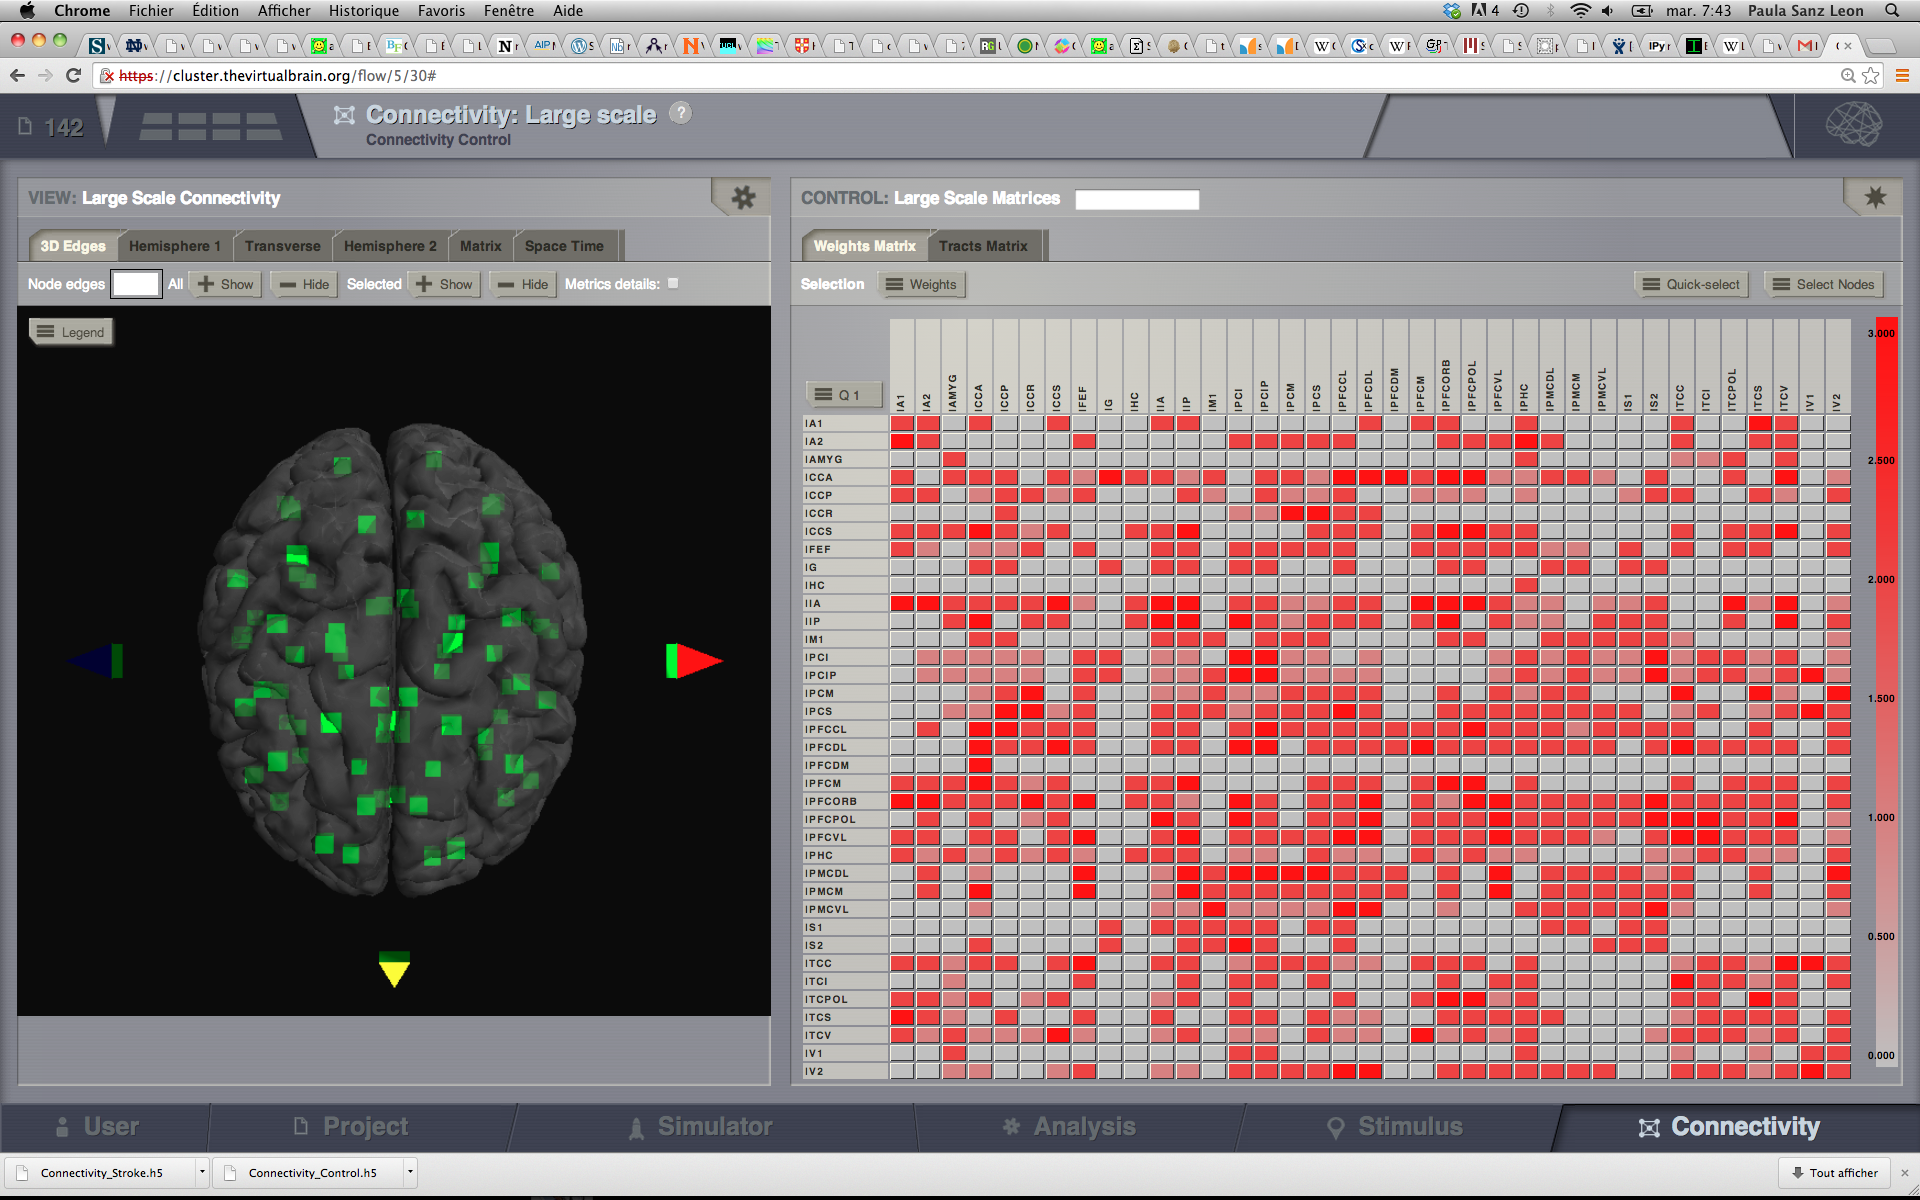
\includegraphics[width=\linewidth]{Handout_UI_ModellingStructuralLesions_ConnectivityArea}%
  \caption{Long-range connectivity editor}%
  \label{fig:fig}%
\end{figure}

\noindent As a first step, we will explore the default connectivity (e.g., go through
the visualizers). To model lesions, we will modify the connectivity, for
instance, by deleting edges or nodes. As a working example we will remove the
interhemispheric connections. 


\begin{formal}
  \begin{enumerate}
  \item Select the left nodes from the \underline{Quick Select} menu. 
  \item Apply the changes. The active or selected nodes will appear in green on the left. 
  \item Save the selection for later use. The connectivity editor will be aware of two set of nodes: those in the selection (green) and those that have not been selected (white). 
  \item Move to the third quadrant (Q3). On the left you can zoom in and draw the connections by selecting a node and then right clicking on it. (Fig. \ref{fig:steps_01_02_03_04})
\end{enumerate}
\end{formal}


\begin{figure}%
  \fbox{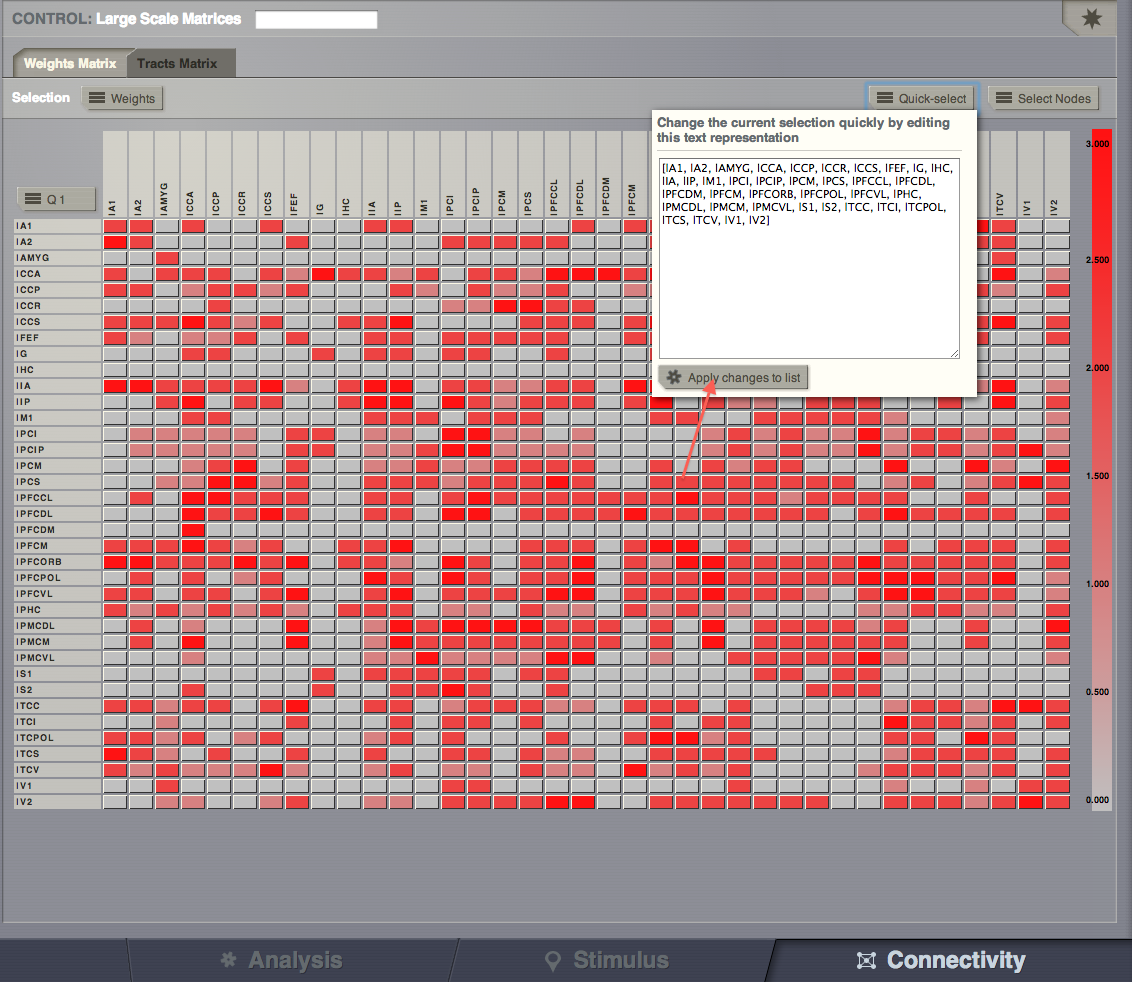
\includegraphics[width=0.75\linewidth]{Handout_UI_ModellingStructuralLesions_SelectLeftNodes.png}}\\
  \fbox{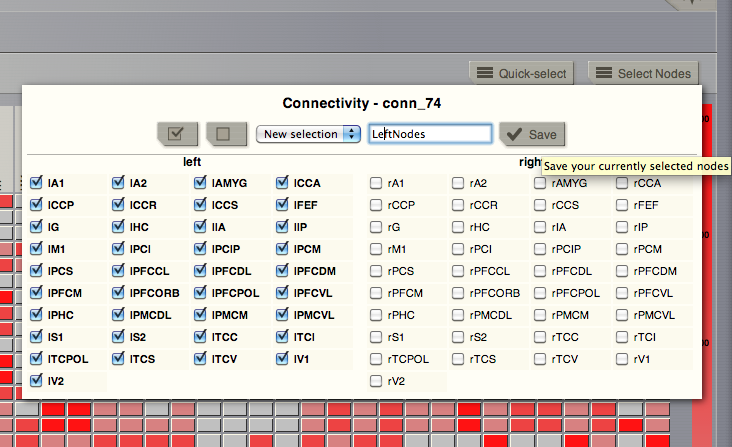
\includegraphics[width=0.75\linewidth]{Handout_UI_ModellingStructuralLesions_SaveLeftNodes}}\\
  \fbox{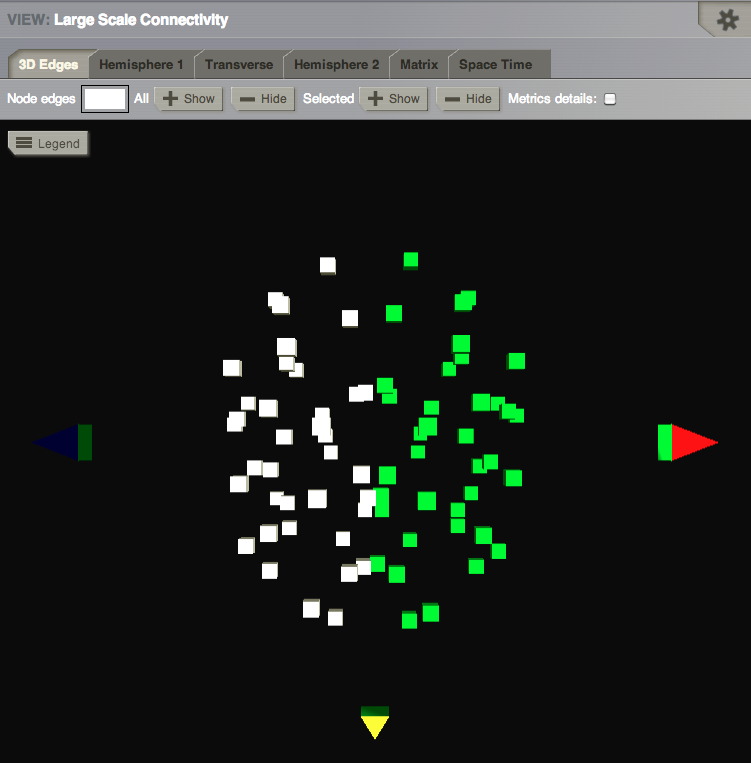
\includegraphics[width=0.75\linewidth]{Handout_UI_ModellingStructuralLesions_SelectedNodes}}\\
  \fbox{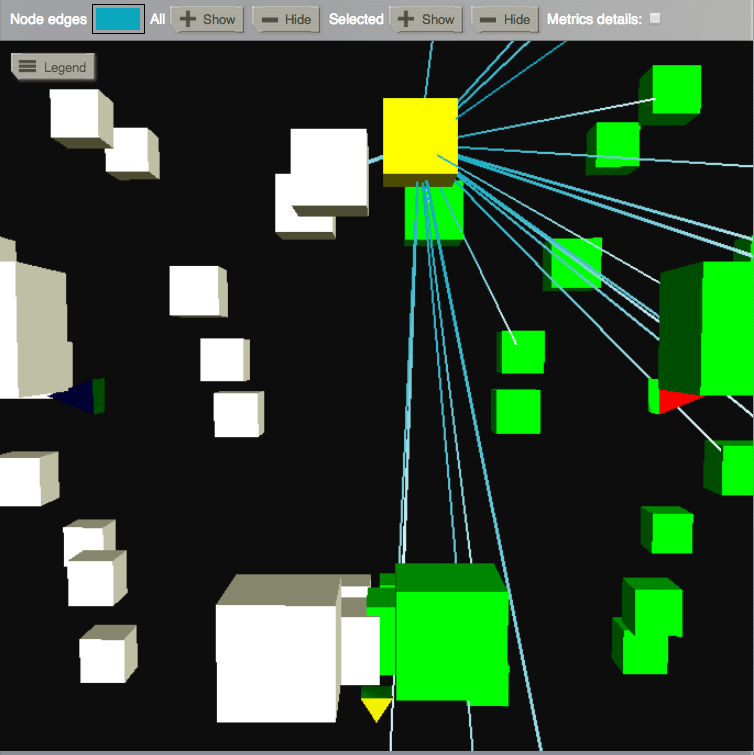
\includegraphics[width=0.75\linewidth]{Handout_UI_ModellingStructuralLesions_DrawConnections}}
  \caption{Edit and save node selection. Draw connections.}
  \label{fig:steps_01_02_03_04}
\end{figure}


\noindent Now we'll proceed to perform operations on the edge values. There are four
edge category of edges depending on the nodes they connect:

\begin{itemize}
  \item Edges IN-IN. These edges connect pair of nodes in the selected set. In this
  particular case you would modify the edges from the left hemisphere.
  \item Edges OUT-OUT. These edges connect pair of nodes in the \textit{unselected
  set}. In this case they would be the right intrahemispheric edges.
  \item Edges IN-OUT. These are the edges that connect nodes in the selected set
  (rows) to nodes in the unselected set (columns). In this case it refers to
  the edges in the second quadrant (Q2).
  \item Edges OUT-IN. These edges connect nodes in the unselected set (rows) to
  nodes in the selected set (columns). In this case it refers to the edges in the third
  quadrant (Q3).
\end{itemize}

\begin{formal}
  \begin{enumerate}[resume]
  \setcounter{enumi}{4}
  \item Select operation \textbf{Set(n)} for edges OUT-IN, set the value to 0 and then apply the changes. 
  \item Select operation \textbf{Set(n)} for edges IN-OUT, set the value to 0 and then apply the changes. (Fig. \ref{fig:steps_05_06})
  \end{enumerate}
\end{formal}


\begin{figure}%
  \fbox{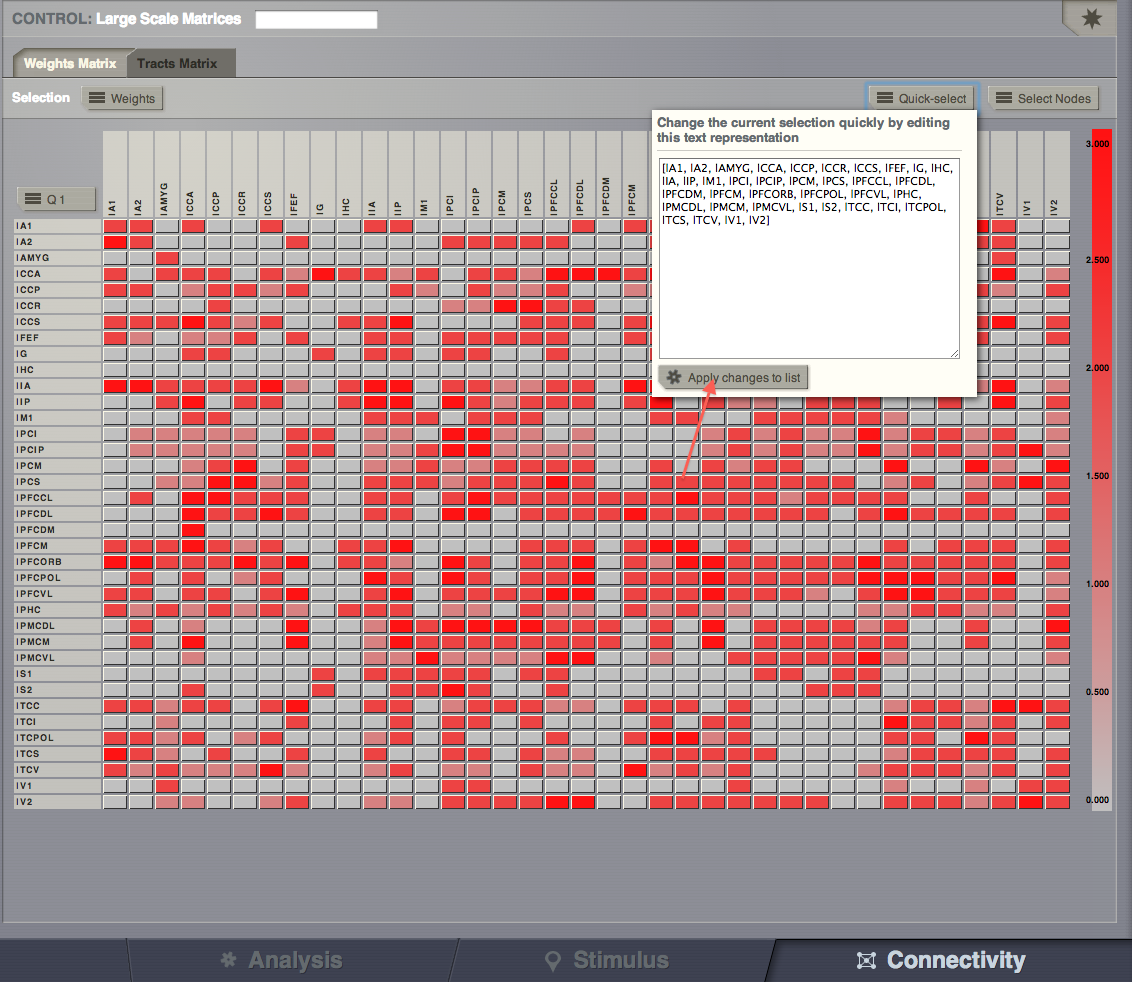
\includegraphics[width=0.75\linewidth]{Handout_UI_ModellingStructuralLesions_SelectLeftNodes.png}}\\
  \fbox{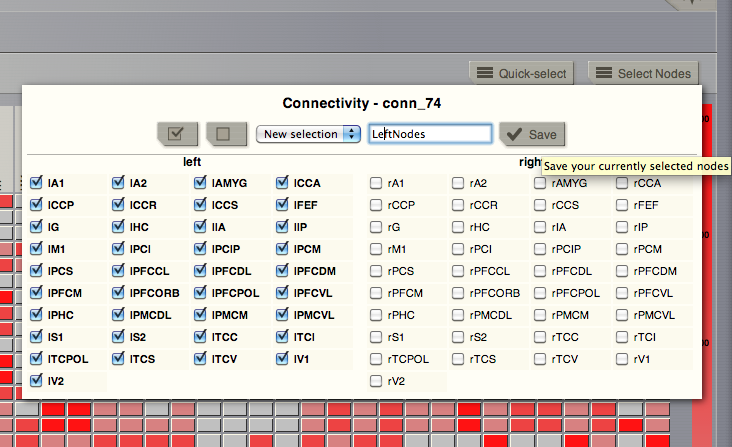
\includegraphics[width=0.75\linewidth]{Handout_UI_ModellingStructuralLesions_SaveLeftNodes}}\\
  \fbox{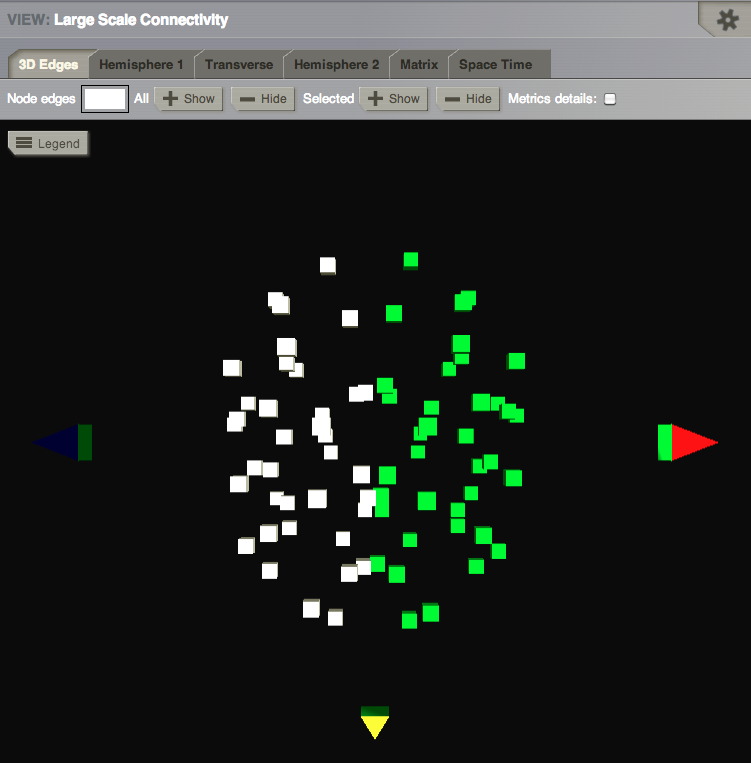
\includegraphics[width=0.75\linewidth]{Handout_UI_ModellingStructuralLesions_SelectedNodes}}\\
  \fbox{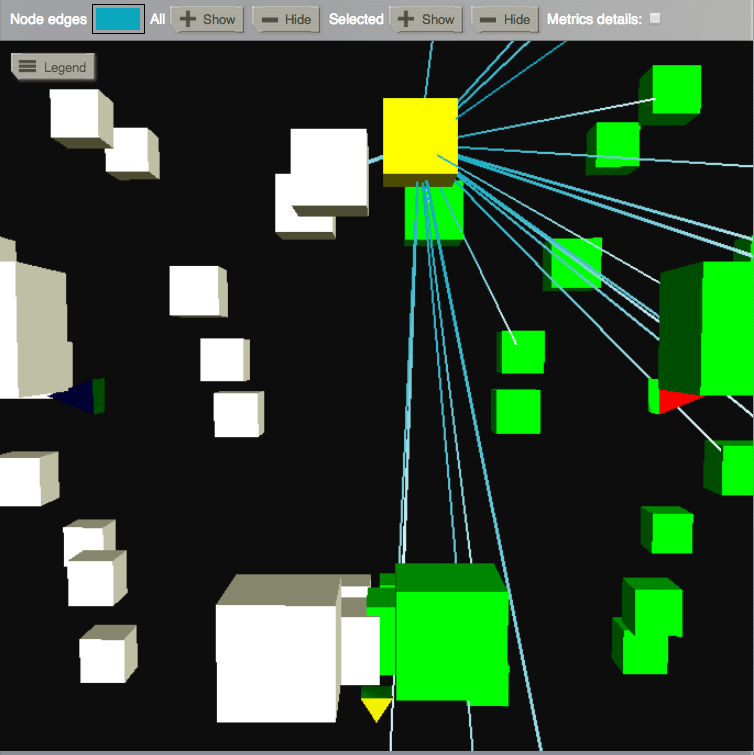
\includegraphics[width=0.75\linewidth]{Handout_UI_ModellingStructuralLesions_DrawConnections}}
  \caption{Edit and save node selection. Draw connections.}
  \label{fig:steps_01_02_03_04}
\end{figure}


\begin{figure}[h]
  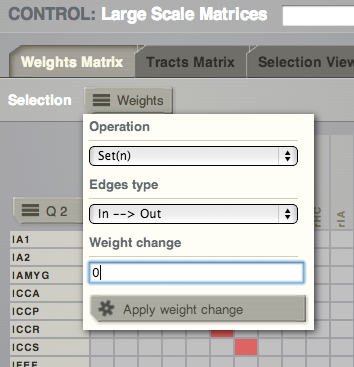
\includegraphics[width=\linewidth]{Handout_UI_ModellingStructuralLesions_EdgeOperations}%
  \caption{Set interhemispheric connections to 0}%
  \label{fig:steps_05_06}%
\end{figure}



\noindent In the matrix editor the interhemispheric connections are gone.
We'll now save the new matrix, but before make sure all the nodes are
included, otherwise TVB will assume you only want the nodes in the current
selection and will set the rest to zero. In the connectivity editor, the nodes
that are not in the selection appear as if they were switched off. (Fig. \ref{fig:steps_save})

\begin{figure}%
  \fbox{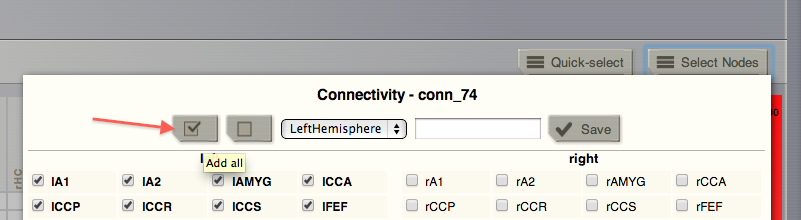
\includegraphics[width=0.75\linewidth]{Handout_UI_ModellingStructuralLesions_SelectAllNodes}}\\
  \fbox{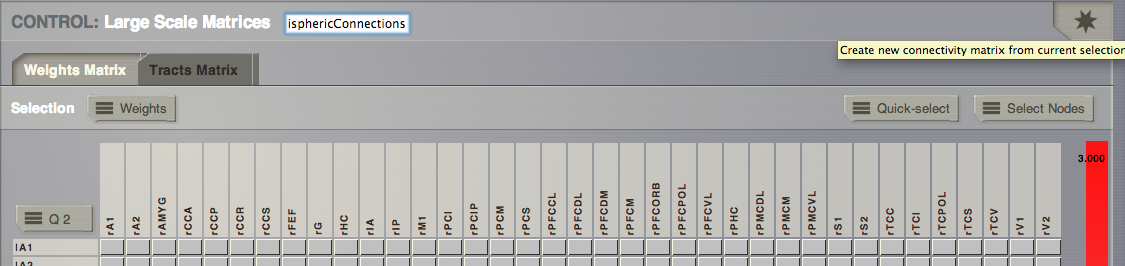
\includegraphics[width=0.75\linewidth]{Handout_UI_ModellingStructuralLesions_SaveNewMatrix}}
  \caption{Select all nodes and save}
  \label{fig:steps_save}
\end{figure}


\begin{formal}
  \begin{enumerate}[resume]
  \setcounter{enumi}{6}
    \item Load the new matrix. (Fig. \ref{fig:steps_07})
  \end{enumerate}
\end{formal}

\begin{figure}[h]
  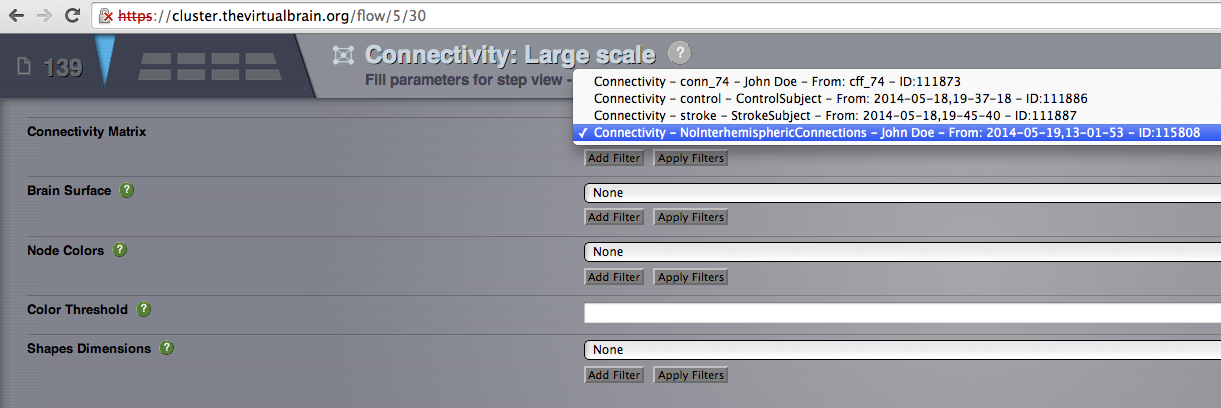
\includegraphics[width=\linewidth]{Handout_UI_ModellingStructuralLesions_LoadNewMatrix}%
  \caption{Set interhemispheric connections to 0}%
  \label{fig:steps_07}%
\end{figure}

\noindent Next, we'll use a criterion based on graph-metrics to select which
nodes will be deleted. Using the BCT \sidenote{Brain Connectivity Toolbox}
algorithms in \underline{\textbf{Analysis}} we compute some degree and
similarity measures and decide to remove the first 5 nodes with the highest
in-strength.


\begin{figure}[h]
  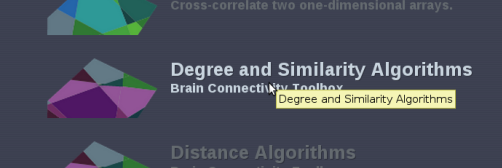
\includegraphics[width=\linewidth]{Handout_UI_ModellingStructuralLesions_Analysis}%
  \caption{Compute network metrics}%
  \label{fig:step_01}%
\end{figure}

%%%%%%%%%%%%%%%%%%%%%%%%%% STEPS %%%%%%%%%%%%%%%%%%%%%%%%%%%%%%%%%%%%%
\begin{formal}
  \begin{enumerate}[resume]
  \setcounter{enumi}{7}
  \item Select degree and similarity algorithms. 
  \item Select the metric you want to compute and the connectivity matrix used as input. Click on launch. 
  \end{enumerate}
\end{formal}
%%%%%%%%%%%%%%%%%%%%%%%%%%%%%%%%%%%%%%%%%%%%%%%%%%%%%%%%%%%%%%%%%%%%%


\noindent By default the last action will take you back to the Operations dashboard.
Once the algorithm is finished, you can see the results in a 2D layout of the
head, which gives an idea of the network topology based on the node-wise
metrics. Alternatively you can display the results as a histogram. 

%%%%%%%%%%%%%%%%%%%%%%%%%% STEPS %%%%%%%%%%%%%%%%%%%%%%%%%%%%%%%%%%%%%
\begin{formal}
  \begin{enumerate}[resume]
  \setcounter{enumi}{9}
  \item Click on 
\includegraphics[width=0.042\linewidth]{nodeConnectivityMeasure}. On
  the overlay window you can already see a summary of the basic descriptive
  statistics (Fig.~\ref{fig:step_02}).

  \item From the Visualizers tab launch the Topographic View.
  \end{enumerate}
\end{formal}
%%%%%%%%%%%%%%%%%%%%%%%%%%%%%%%%%%%%%%%%%%%%%%%%%%%%%%%%%%%%%%%%%%%%%

\begin{figure}[h]
  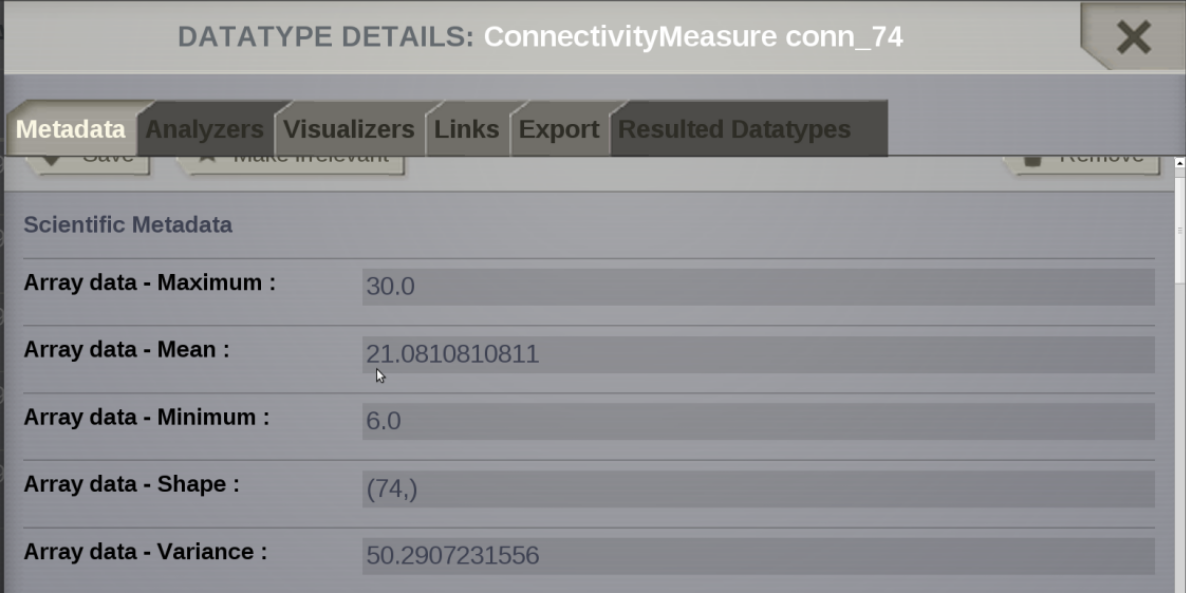
\includegraphics[width=\linewidth]{Handout_UI_ModellingStructuralLesions_AnalysisResult}%
  \caption{Descriptive summary}%
  \label{fig:step_02}%
\end{figure}

%%%%%%%%%%%%%%%%%%%%%%%%%% STEPS %%%%%%%%%%%%%%%%%%%%%%%%%%%%%%%%%%%%%
\noindent Other network measures were previously computed so we can also have a look at them. 
\begin{formal}
  \begin{enumerate}[resume] %% doesnt work with the formal enviornment :/
  \setcounter{enumi}{11}
  \item Select strength and clustering coefficient from the brain menu (Fig. ~\ref{fig:step_05}). Click on \underline{Update Visualizer}.
  \end{enumerate}
\end{formal}
%%%%%%%%%%%%%%%%%%%%%%%%%%%%%%%%%%%%%%%%%%%%%%%%%%%%%%%%%%%%%%%%%%%%%
\noindent It is possible to view and compare up to three metrics (Fig. ~\ref{fig:step_05b}).
\begin{figure}[h]
  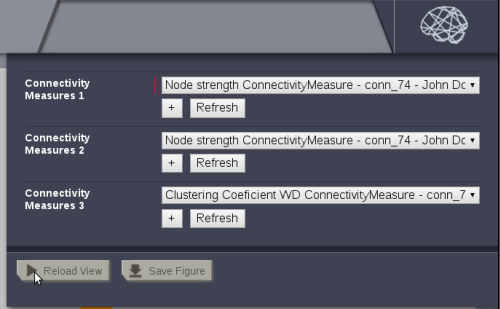
\includegraphics[width=0.5\linewidth]{Handout_UI_ModellingStructuralLesions_AnalysisView}%
  \caption{Select additional network metrics}%
  \label{fig:step_05}%
\end{figure}

\begin{figure}[h]
  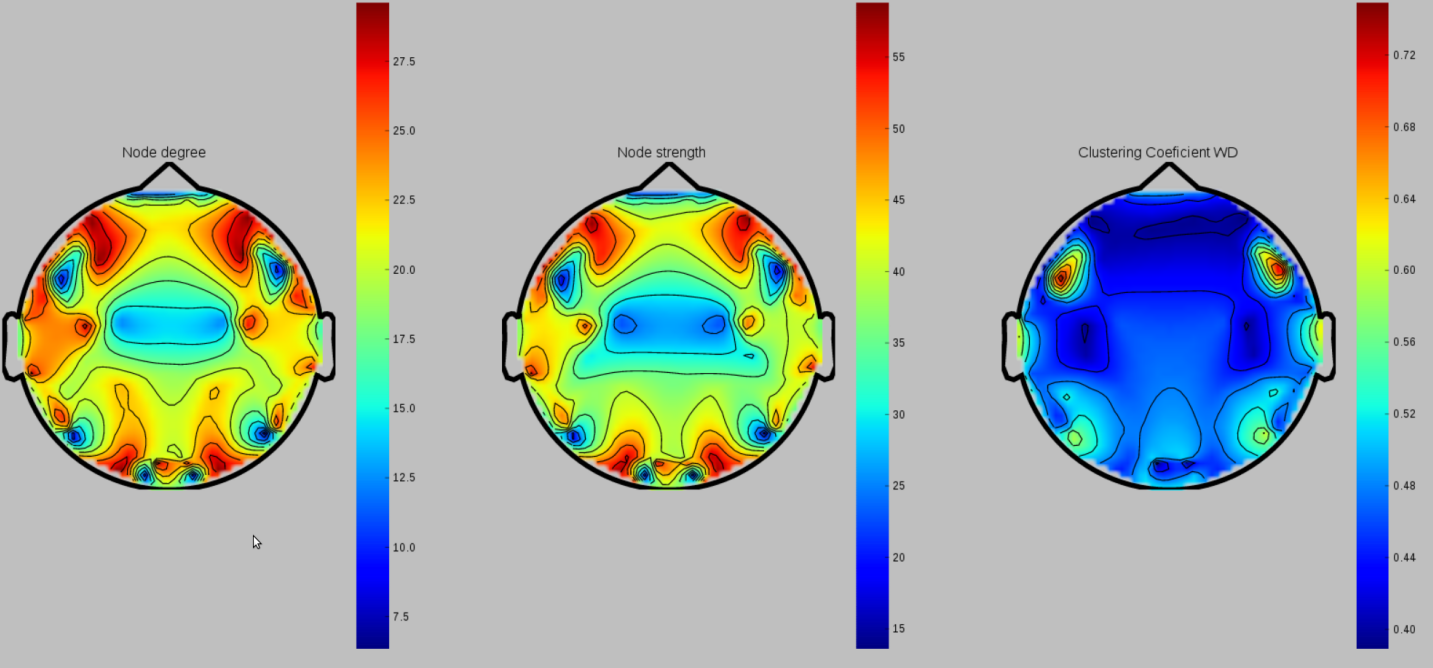
\includegraphics[width=0.9\linewidth]{Handout_UI_ModellingStructuralLesions_AnalysisResultCompare}%
  \caption{View and compare network metrics}%
  \label{fig:step_05b}%
\end{figure}
\newpage

\noindent We go back to the \textsc{Connectivity} area and in the field \underline{Node colours} we select
the node-wise metric we just computed and set a threshold of 56. Launch the connectivity editor.

\begin{formal}
  \begin{enumerate}[resume] %% doesnt work with the formal enviornment :/
  \setcounter{enumi}{12}
  \item Go to the Transverse visualizer wich displays a spring-like layout of the network graph (top view). Clikc on \underline{Show all} to apply the threshold previously set. Fig. \ref{fig:step_12}
  \end{enumerate}
\end{formal}

\begin{figure}[h]
  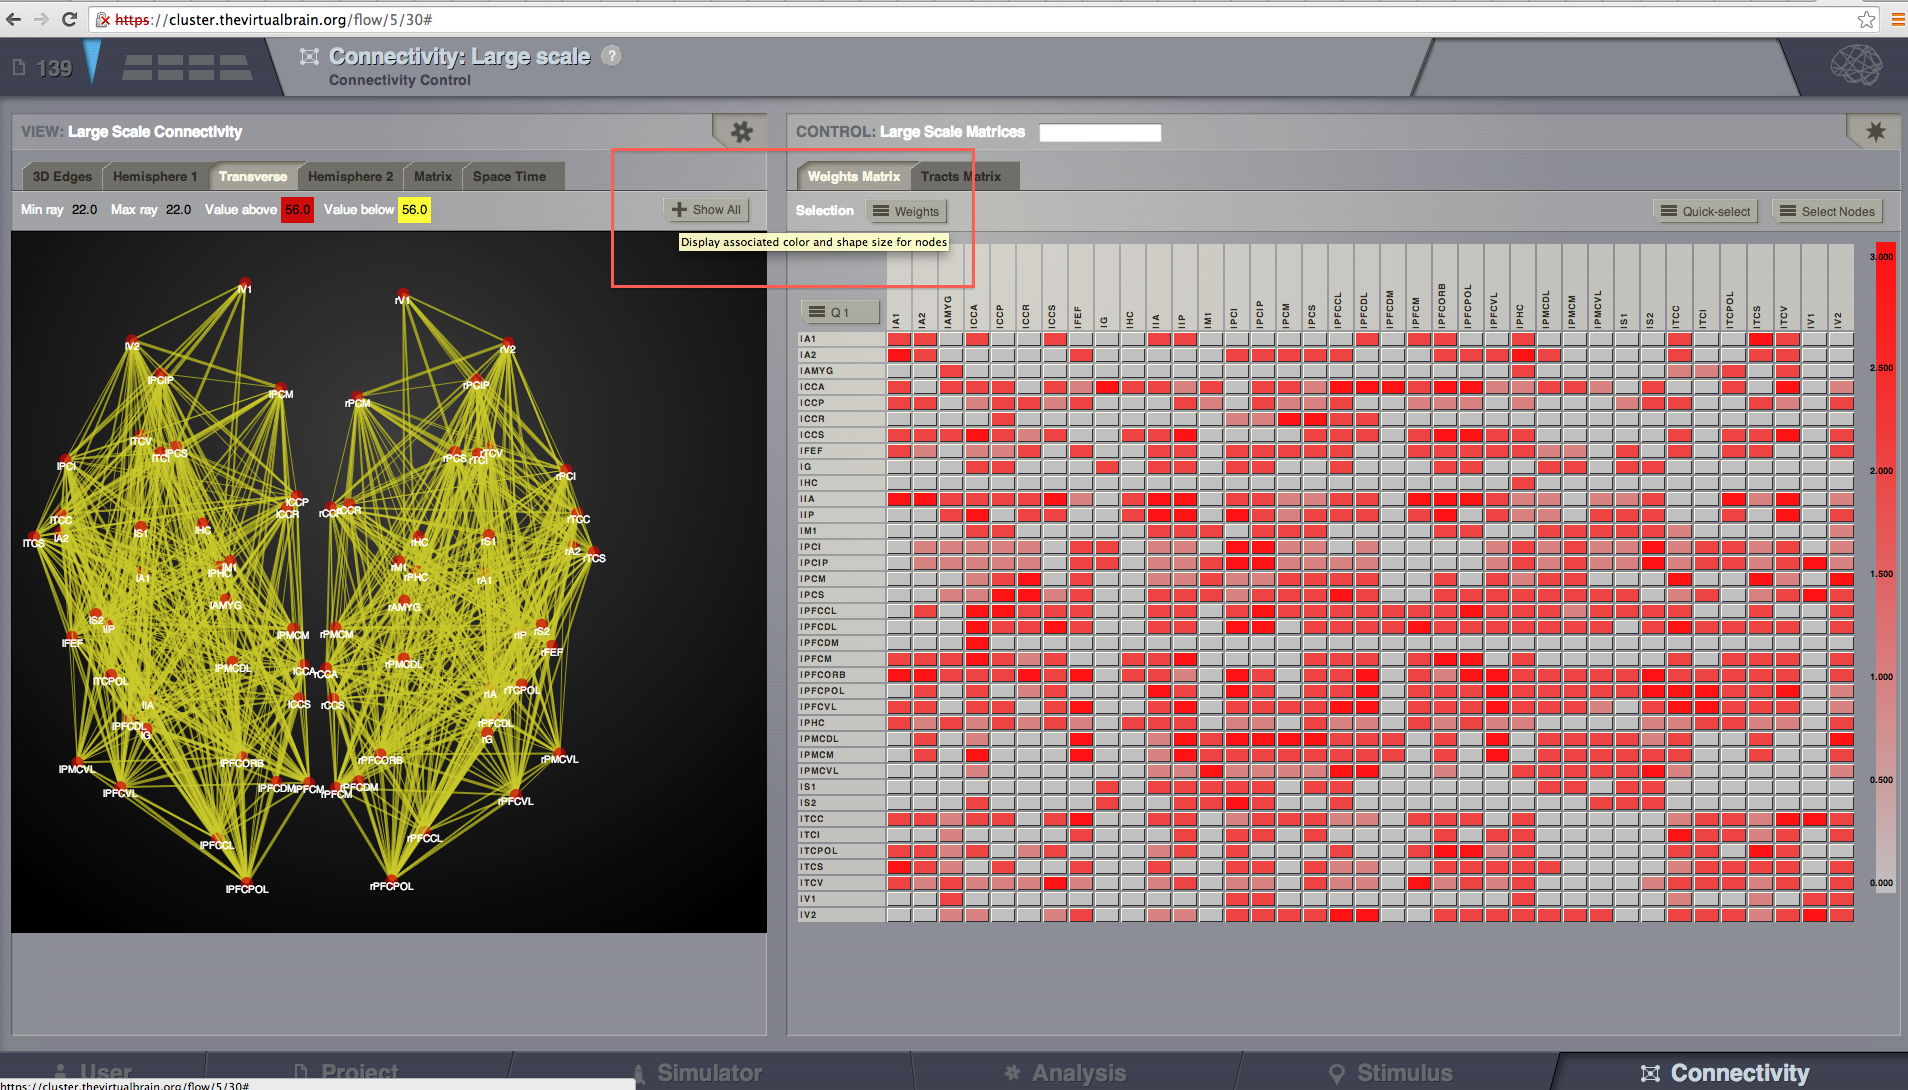
\includegraphics[width=0.9\linewidth]{Handout_UI_ModellingStructuralLesions_ShowColourNodes}%
  \caption{Show node colours.}%
  \label{fig:step_12}%
\end{figure}
\newpage

To completely remove the nodes we could create a selection excluding these
high-degree nodes nodes and save the new matrix, or creating a small selection
with the target nodes and using the edge operations we set the edges of the
IN-IN, IN-OUT and OUT-IN to zero. (Fig. \ref{fig:step_subnetwork})


\begin{figure}[h]
  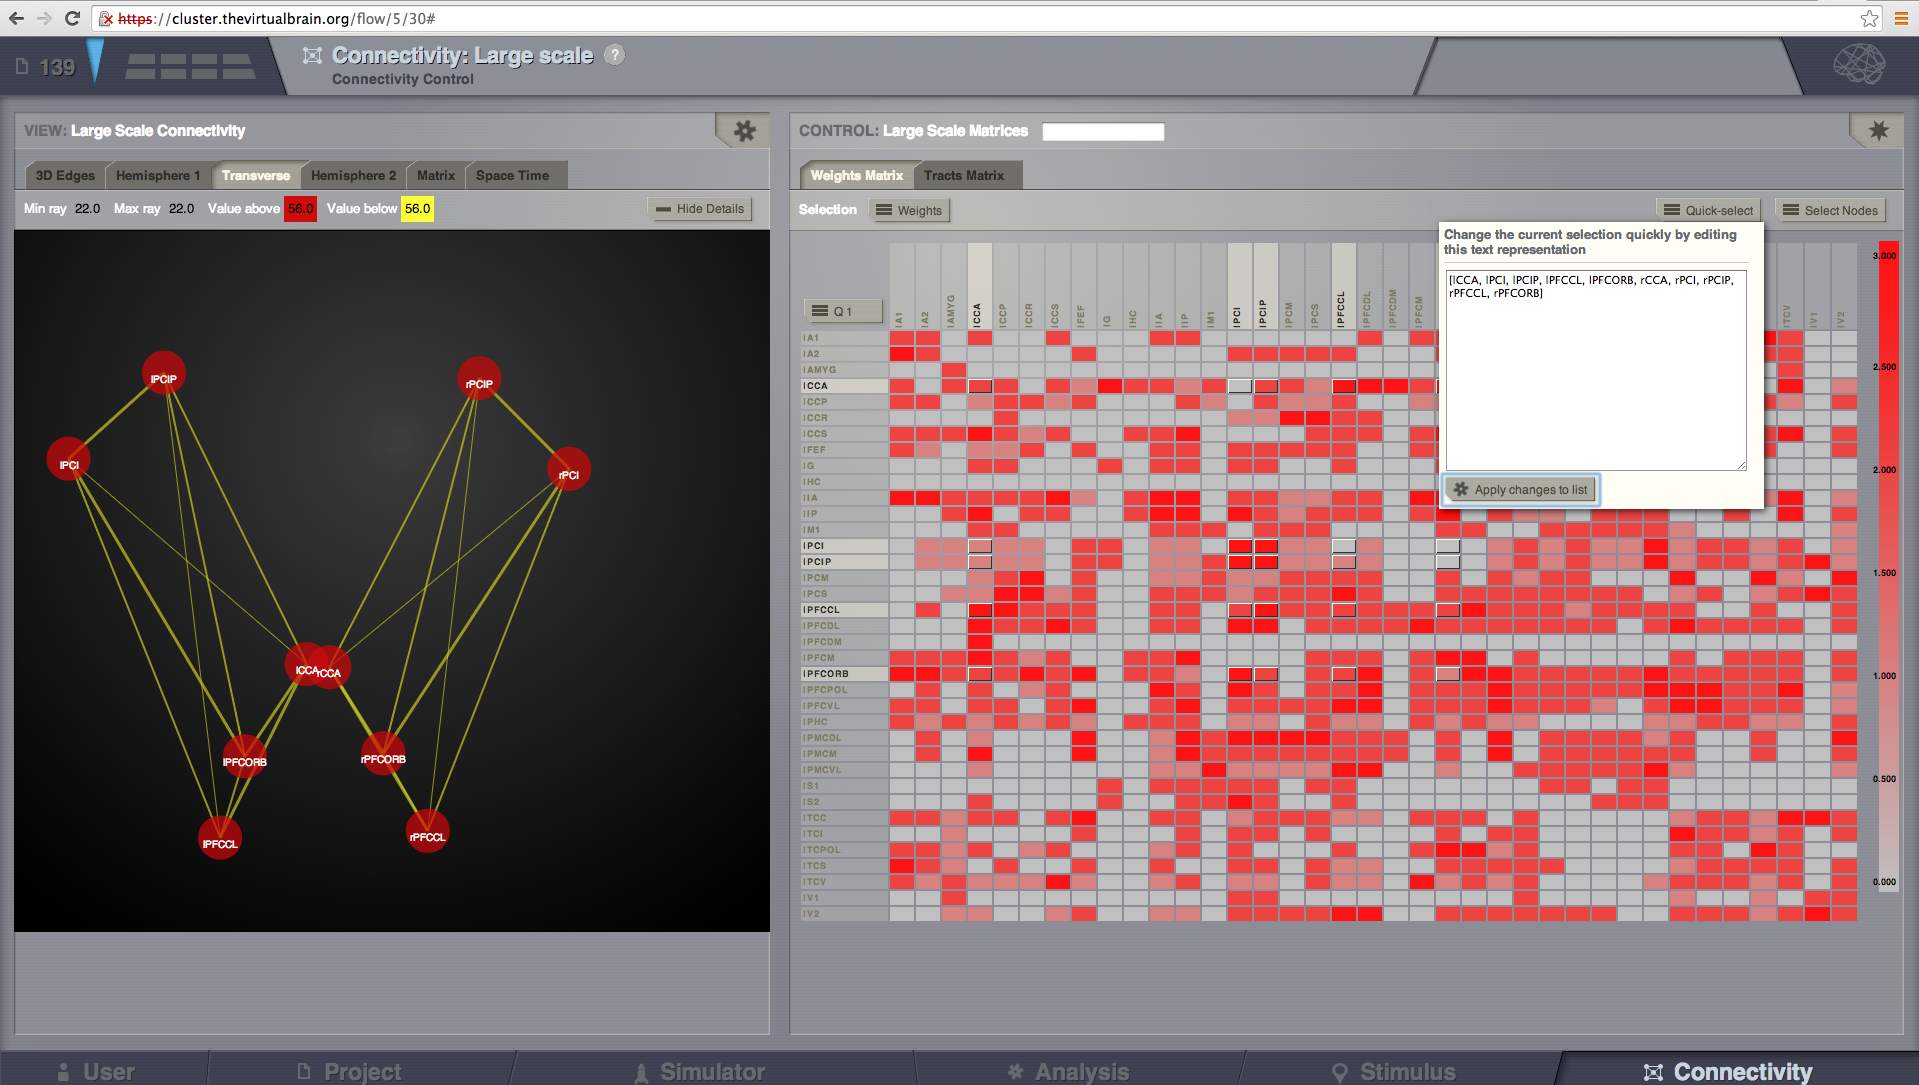
\includegraphics[width=0.9\linewidth]{Handout_UI_ModellingStructuralLesions_SelectSubnetwork}%
  \caption{Select subnetwork with the highest in-strength nodes.}%
  \label{fig:step_subnetwork}%
\end{figure}
\newpage


We could repeat from step 13 on using a different metric. From the \underline{Brain menu}
 you can change the measure used to colour the nodes as well as the threshold. Fig. \ref{fig:step_change_threshold}

\begin{figure}[h]
  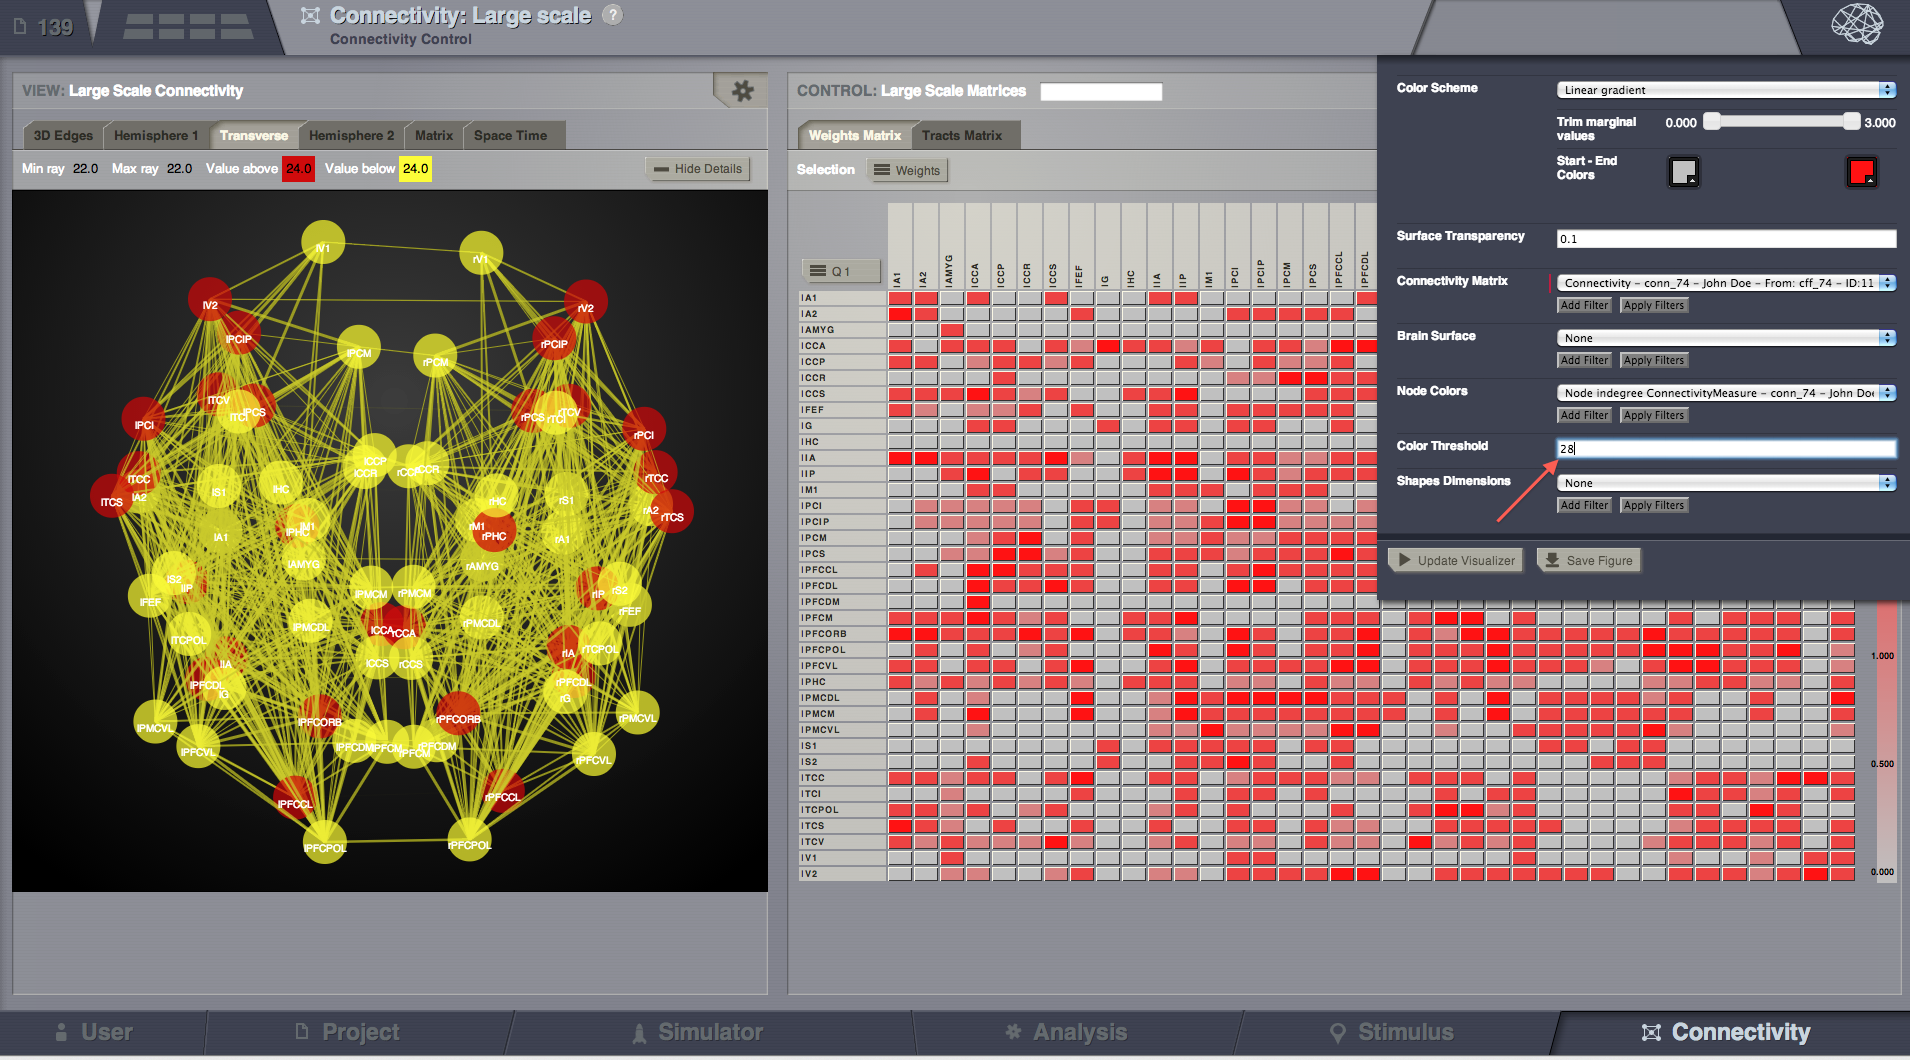
\includegraphics[width=0.9\linewidth]{Handout_UI_ModellingStructuralLesions_ChangeNodeColourThreshold}%
  \caption{Change the metric and threshold.}%
  \label{fig:step_change_threshold}%
\end{figure}
\newpage

\subsection{Steps: Simulation}

\noindent We can now try to evaluate the difference between the activity generated by both the different connectivty matrices. 
Go to the \textsc{simulator} area. Now, we'd like to see how these modifications have altered the stability plane
of our system. Many figures are available in \textsc{Projects} $\rightarrow$ \textsc{Image archive}.

\begin{simulation}
  \begin{enumerate}
  \item We proceed to launch a PSE using the same parameters as in the first session and second PSE where
the only element that has changed is the connectivity matrix.

  \item Select point in the PSE maps (e.g., points with the same parameters). Tag the time-series. Go to \textsc{Analysis} $\rightarrow$ \textsc{Fourier spectrum}. Apply a filter to find your the time-series and launch the analyzer. Fig. \ref{fig:steps_sim_03}.

  \item We can now compare the results.

  \item In addition we explore the model presented in the previous talk (Stefanescu-Jirsa 3D) using the control and stroke connectivity matrices. 
  \item Select a point from each PSE map. Tag the corresponding time-series. Launch the \underline{Animated time-series visualizer}. Apply a filter to find the interesting traces. 

  \item Then using the parameters from these points, we launch two 60 seconds long simulations using the BOLD monitor to have a proper history for our actual simulation. (This was done for both models). 

  \item Using the branching mechanims, we launch 4 minutes simulations and compute the Pearson correlation coefficients matrix. (Fig. \ref{fig:steps_sim_07}) 

  \end{enumerate}
\end{simulation}


\begin{figure}%
  \fbox{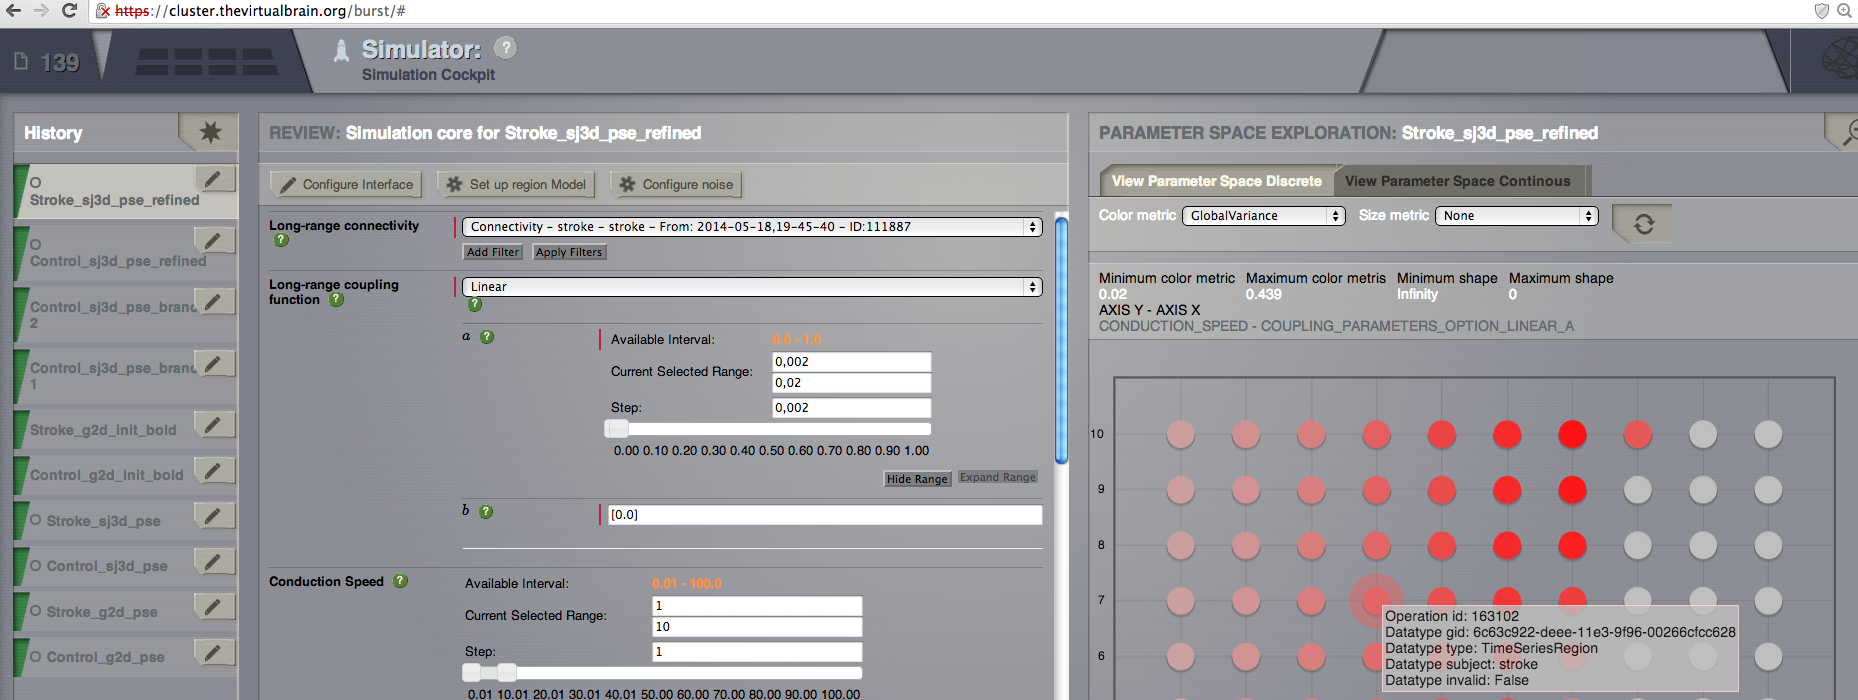
\includegraphics[width=0.82\linewidth]{Handout_UI_ModellingStructuralLesions_SelectPointFromPSE_a}}\\
  \fbox{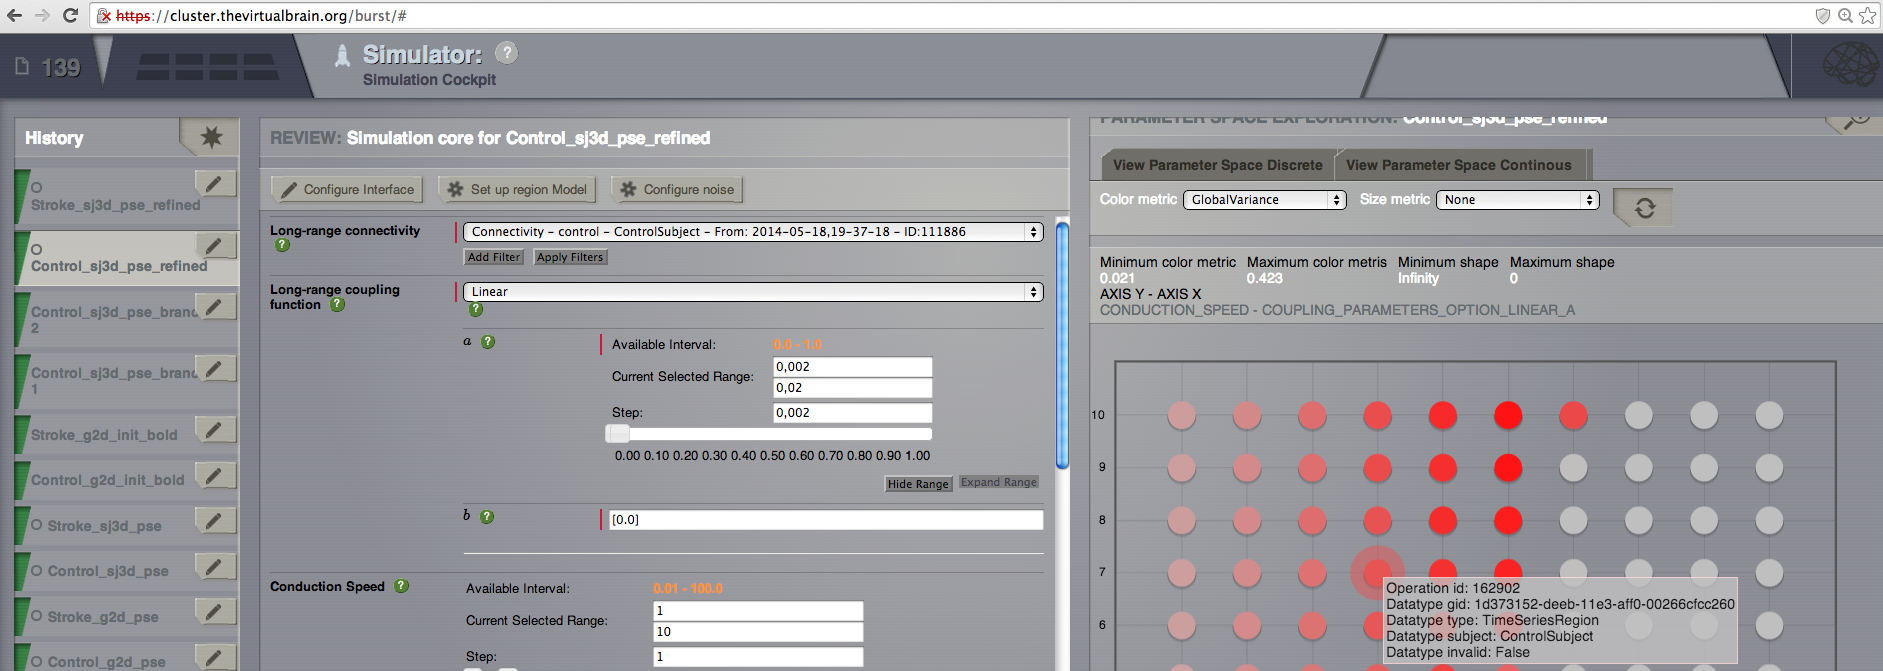
\includegraphics[width=0.82\linewidth]{Handout_UI_ModellingStructuralLesions_SelectPointFromPSE_b}}
  \caption{Select points}
  \label{fig:steps_sim_03}
\end{figure}


\begin{figure}%
  \fbox{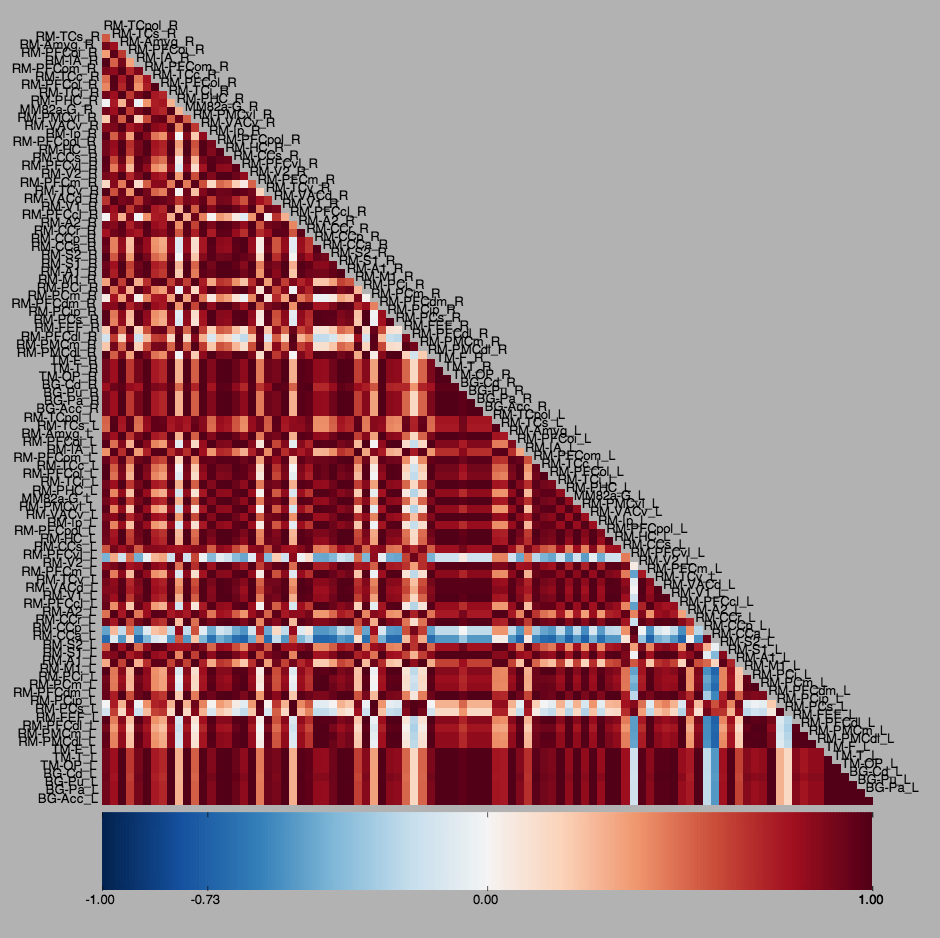
\includegraphics[width=0.82\linewidth]{Handout_UI_ModellingStructuralLesions_bold_pearson_g2d_control}}\\
  \fbox{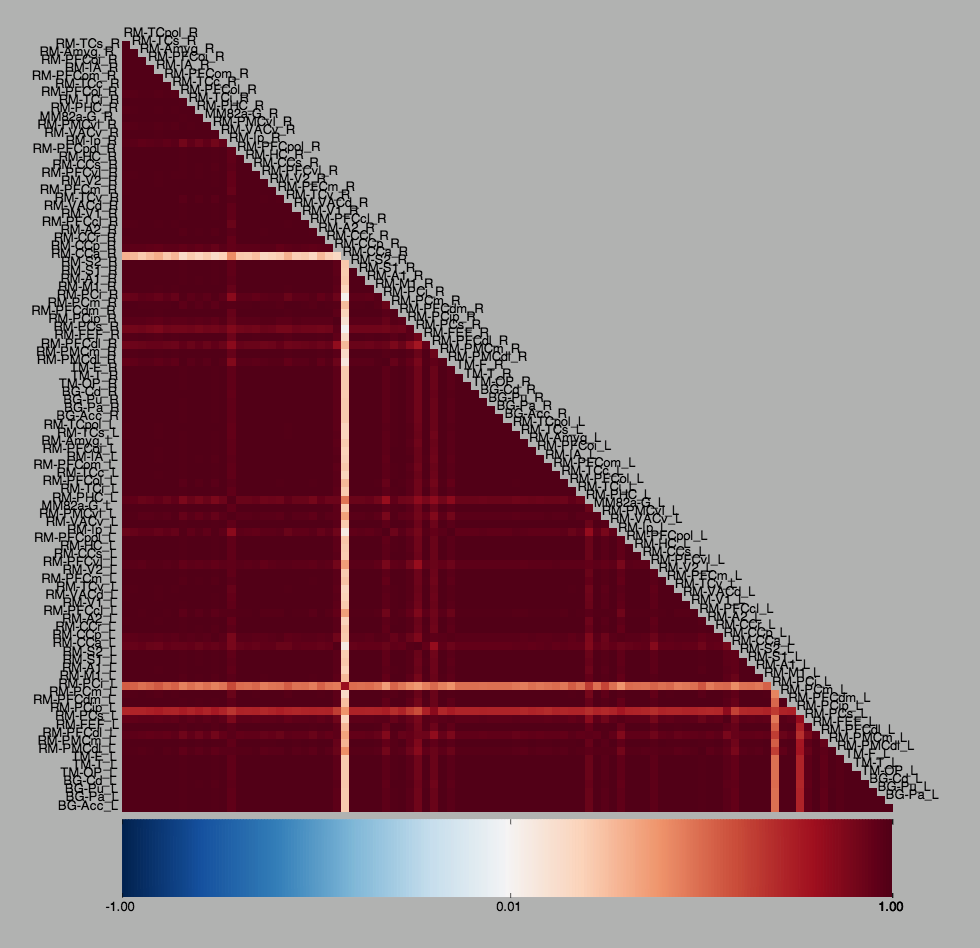
\includegraphics[width=0.82\linewidth]{Handout_UI_ModellingStructuralLesions_bold_pearson_g2d_stroke}}
  \caption{Pair-wise Pearson correlation coefficient matrix computed over the long BOLD time-series. Top: control matrix. Bottom: stroke matrix.}
  \label{fig:steps_sim_07}
\end{figure}



% \section{Results}\label{sec:results}
% If the time-series were processed in matlab or python to obtain certain
% figures like Fig.~\ref{fig:fig_results}, then they should be reproducible.
% Provide a code snippet to reproduce the figure. Add some conclusions.

% \begin{figure}[h]
%   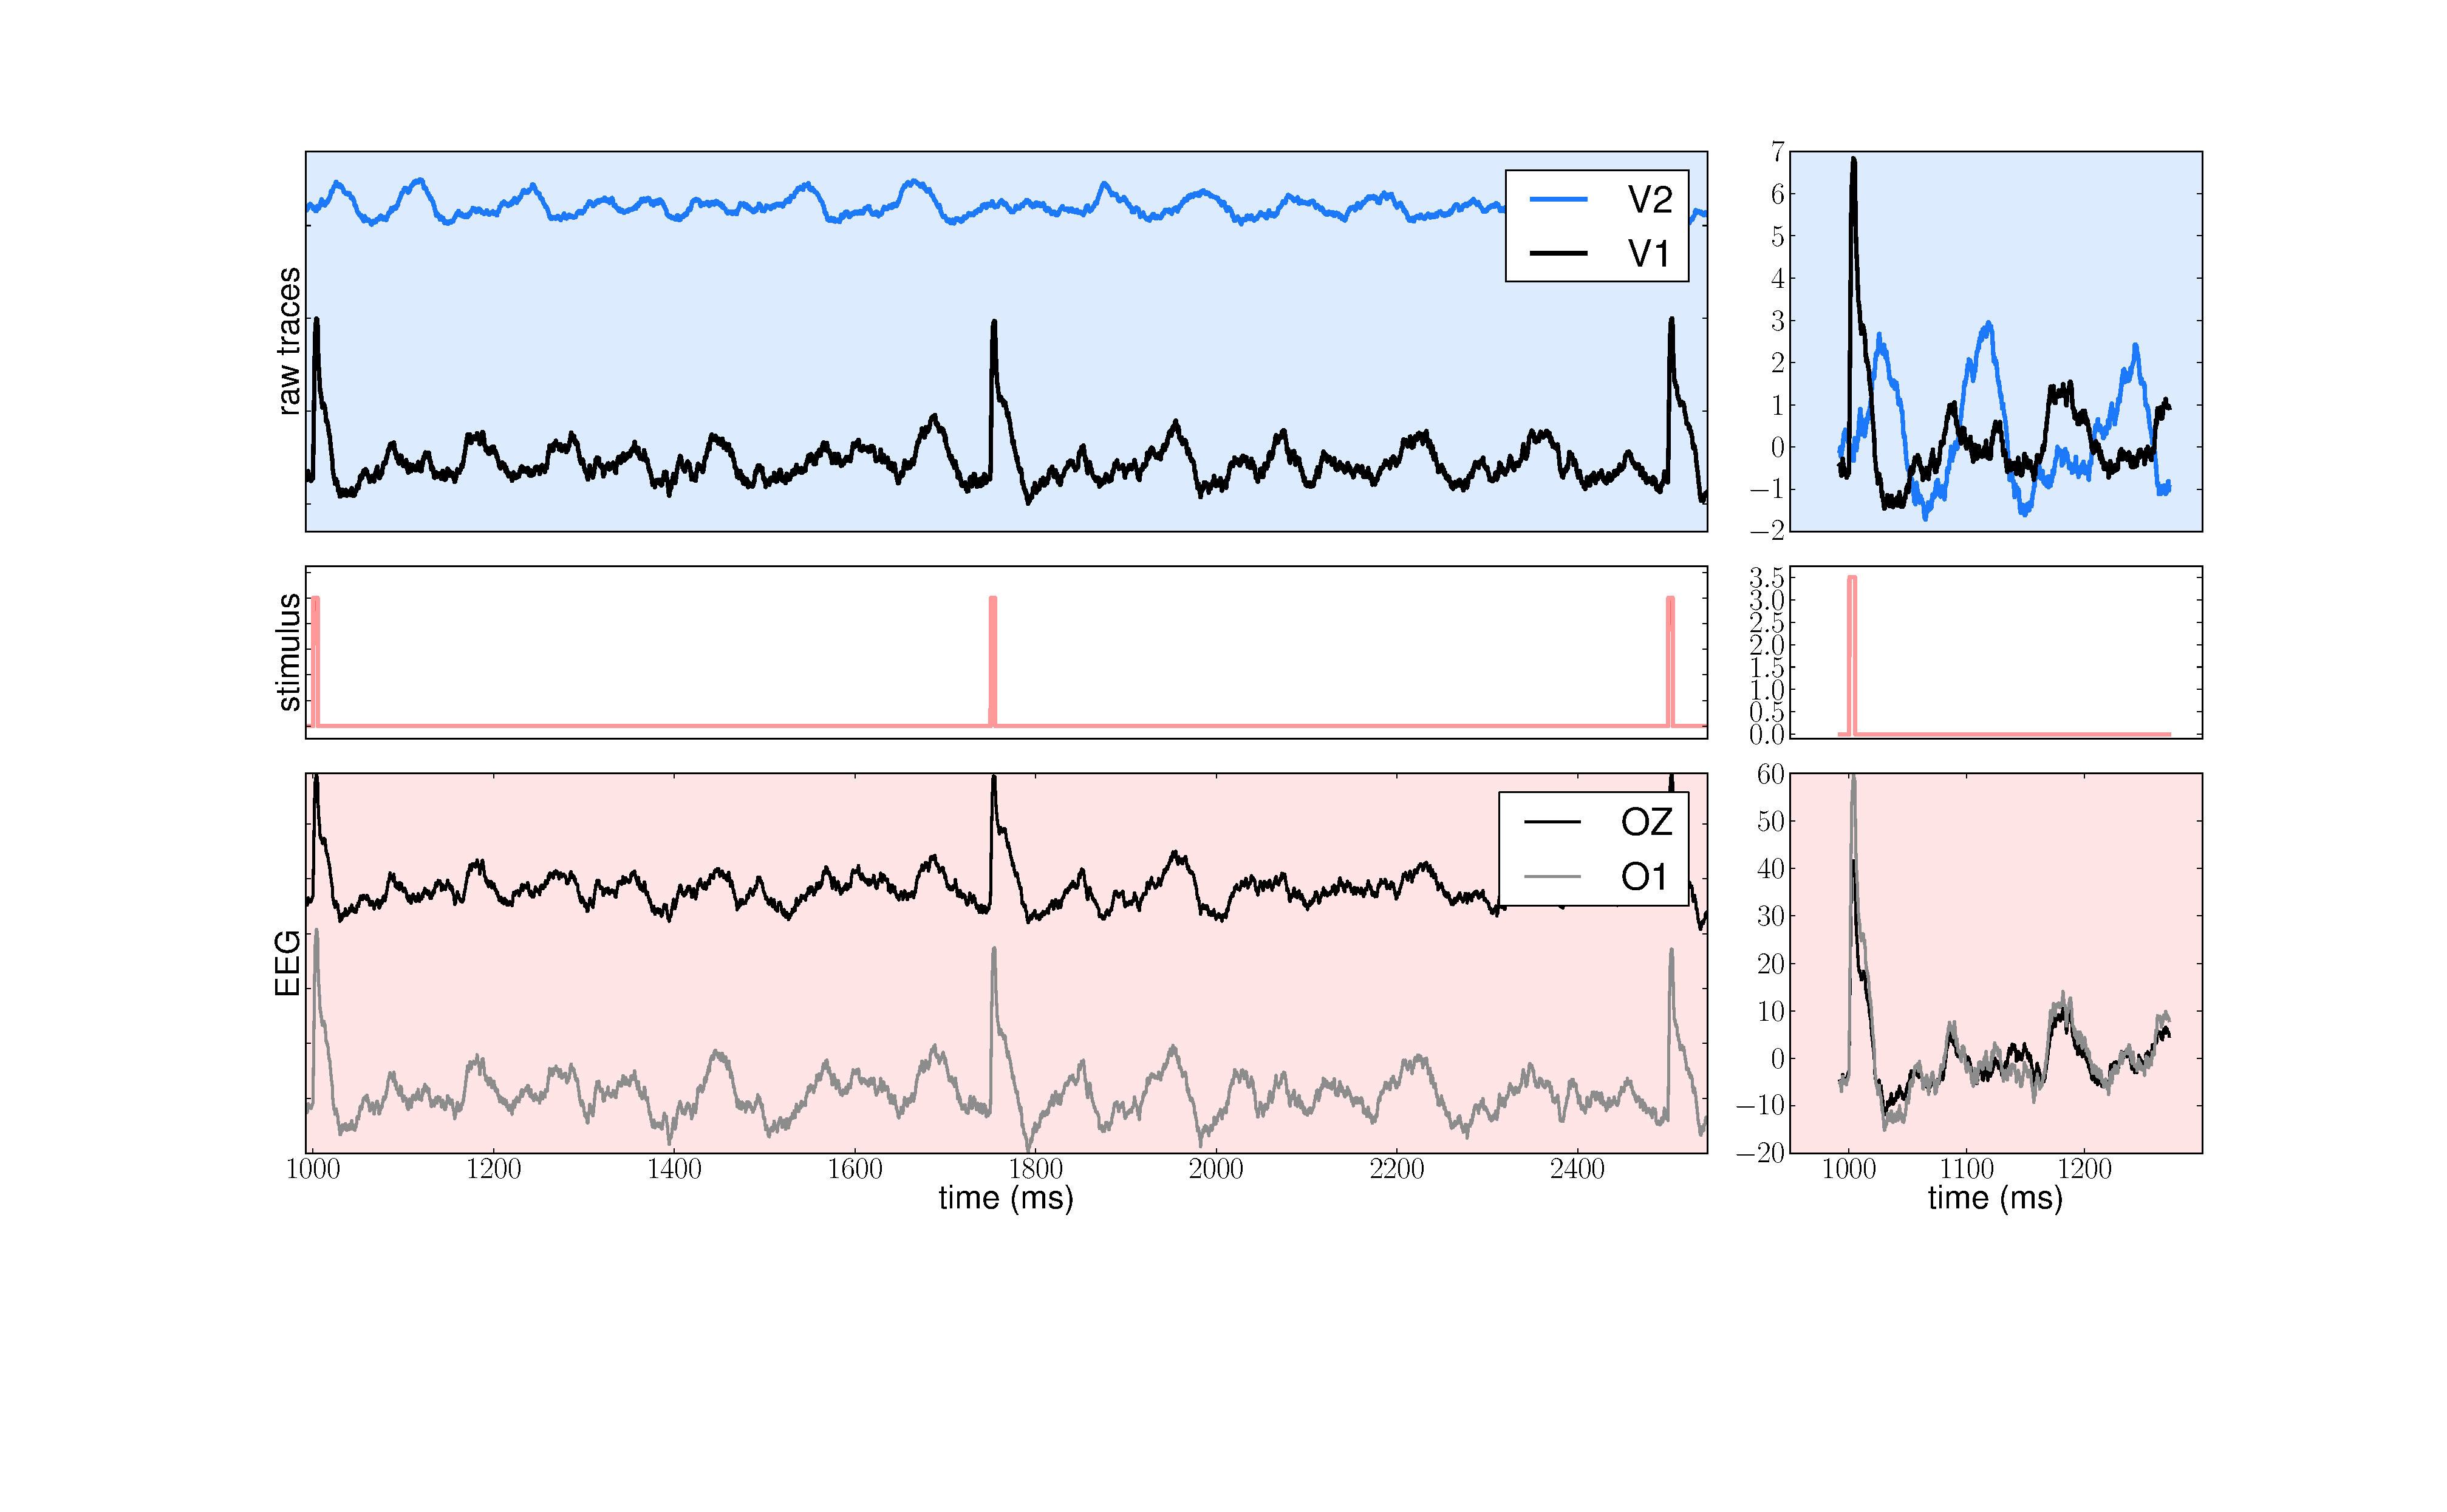
\includegraphics[width=\linewidth]{results_Example_ER_stochastic.pdf}%
%   \caption{Long-range connectivity editor}%
%   \label{fig:fig_results}%
% \end{figure}


\section{More Documentation}\label{sec:more-doc}
For more documentation on The Virtual Brain, please see the following articles \cite{Sanz-Leon_2013, Spiegler_2013, Woodman_2014, Jirsa_2010b}


\section{Support}\label{sec:support}

The official TVB webiste is \url{www.thevirtualbrain.org}.  
All the documentation and tutorials are hosted on \url{the-virtual-brain.github.io}.
You'll find our public \smallcaps{git} repository at \url{https://github.com/the-virtual-brain}. 
For questions and bug reports we have a users group \url{https://groups.google.com/forum/#!forum/tvb-users}

\bibliography{tvb_references}
\bibliographystyle{plainnat}

\end{document}